\section{Callbacks}
Javascript ist eine auf Events basierende Programmiersprache. Das bedeutet, anstatt auf blockierenden Code zu warten, führt Javascript Operationen weiter aus und reagiert wenn die Aktion fertig ist. Um sicherzustellen, dass Javascript auf die Fertigstellung von asynchronen Operationen wartet, wurden Callbacks eingeführt. Doch was genau sind Callbacks? \\

\noindent
Sowohl in Javascript als auch in Typescript sind Funktionen als Erste-Klasse-Objekte zu sehen. Aus diesem Grund ist es Möglich sie als Argumente in anderen Funktionen oder als Rückgabewert einzusetzen. Diese übergebenen Funktionen heißen Callbacks und werden dann \glqq{}später\grqq{} innerhalb des Funktionsrumpfes aufgerufen. Callbacks, auch Rückruffunktionen genannt, ist die am meist verbreitetste Technik der funktionalen Programmierung in Javascript.\cite{callbacks-intro} Javascript bietet mit Arrays mitgelieferte Callbacks wie z.B:

\begin{figure}[H]
\begin{lstlisting}
const numbers: number[] = [1, 2, 3, 4, 5, 6];
function isEven(x): boolean { 
  return x % 2 === 0; 
}

const evenNumbers = numbers.filter(isEven);
console.log(evenNumbers) // 2 4 6
\end{lstlisting}
\caption{Die Funktion filter() gibt ein neues Array zurück.\cite{callbacks-example}}
\end{figure}

\noindent
Die Methode filter() nimmt Elemente einer Liste heraus, basierend einer Funktion die, die Filterkonditionen bestimmt. Dabei wird zuerst, dass Element aus der Liste entnommen und dann die Kondition geprüft. Wenn also eine Funktion als Parameter übergeben wird, wird diese nicht sofort ausgeführt. Eine Funktion die ein Callback als Input-Parameter annimmt, wird auch High-Order-Funktion genannt.

\subsubsection{Beispiel}

In dem nächsten Beispiel wird gezeigt, wie asynchrone Operationen sich verhalten, wenn nicht explizit auf die Fertigstellung gewartet wird. Vor dem Ausführen des Beispiels muss folgend konfiguriert werden:

\begin{center}
    Promises-vs.-Observables$\,\to\,$ webpack.config.js
\end{center}

\begin{figure}[H]
\begin{lstlisting}
module.exports = {
    mode: 'development',
    entry: './src/modules/sync-vs-async.ts',
    ...
}
\end{lstlisting}
\caption{Hier sollte vor dem Starten des Projekts die Typescript Datei sync-vs-async.ts als Eingangspunkt definiert werden.}
\end{figure}

\begin{figure}[H]
\begin{lstlisting}
export class Print {

    public msg(msg: string): void {
        document.body.innerHTML +=
            `<div class="alert" role="alert">${msg}</div>`;
    }
}

class Synchronous extends Print {

    public printMessages(): void {
        this.msg('Hey Im message Nr. 1!');
        this.msg('Hey Im message Nr. 2 !');
        this.msg('Hey Im message Nr. 3 !');
        this.msg('Done!');
    }
}

class Asynchronous extends Print {

    public printMessages(): void {
        setTimeout(() => this.msg('Hey Im message Nr. 1 !'), Math.random() * 10);
        setTimeout(() => this.msg('Hey Im message Nr. 2 !'), Math.random() * 10);
        setTimeout(() => this.msg('Hey Im message Nr. 3!'), Math.random() * 10);
        setTimeout(() => this.msg('Done!'), Math.random() * 10);
    }
}

const synchronous = new Synchronous();
const asynchronous = new Asynchronous();

synchronous.printMessages();
asynchronous.printMessages();
\end{lstlisting}
\end{figure}

\noindent
Diese Datei enthält drei Klassen. Während \textbf{Print} als Basisklasse eine Methode für das Addieren einer Nachricht in die HTML-Dom bereitstellt, rufen die abgeleiteten Klassen \textbf{Synchronous} und \textbf{Asynchronous} die Nachricht in verschiedener Weise auf. In der Klasse Synchronous werden die HTML-Elemente sequenziell in die Dom eingefügt. In der Asynchronous Klasse dagegen wird mit Hilfe der Callback-Funktion setTimeout() eine zeitintensive Operation simuliert. Das könnte zum Beispiel ein Aufruf an einem API-Endpunkt sein. Da setTimeout() eine Rückruffunktion ist, die die Antwortzeit verzögert, wird ein neuer Thread eröffnet. Währenddessen führt Javascript schon die nächste Operation aus. Aufgrund der zufällig ausgewählten Zeitverzögerung ist nie klar welche Nachricht als erstes ausgegeben wird. Das heißt die Callback-Aufrufe finden völlig unabhängig voneinander statt. Zeittechnisch bedeutet das, dass in dem synchronen Modell die Zeit für jede ausgeführte Operation addiert wird, während im asynchronen Modell die Zeitfenster völlig unabhängig voneinander laufen. Daraus sollte sich jedoch nicht zurückschließen lassen, dass synchrone Prozessabläufe länger oder schneller zum Verarbeiten brauchen.
Das Ergebnis sieht wie folgt aus:

\begin{figure}[H]
\centering
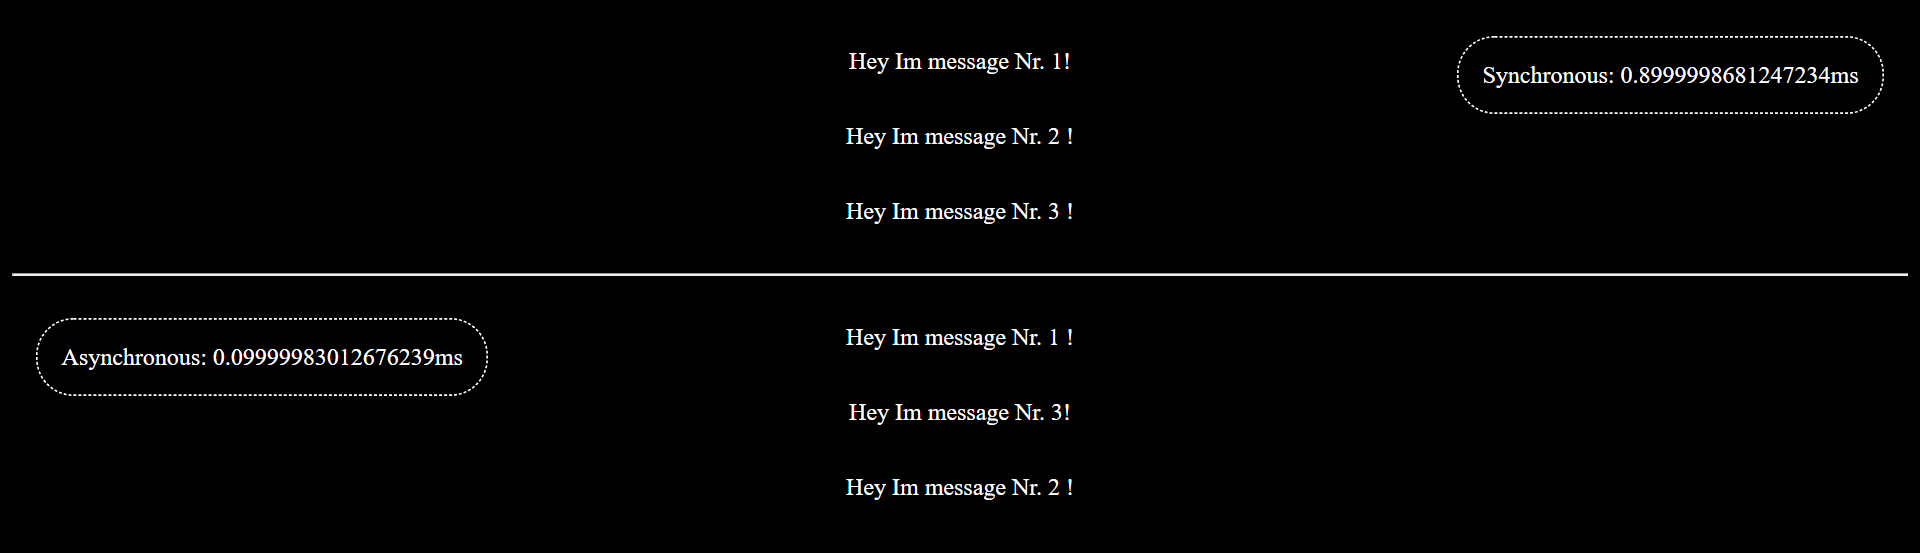
\includegraphics[width=10cm]{synchronous-vs-asynchronous}
\caption{Die Asynchronous Klasse gibt die Nachrichten zufällig aus.}
\end{figure}

\noindent
Zusammenfassend kann man also sagen, dass in dem synchronen Modell implizit auf die Aktionen gewartet wird, und in dem asynchronen Modell explizit. Als Diagramm abgebildet führt der Browser die Methoden wie folgt aus:

\begin{center}
\begin{figure}[H]
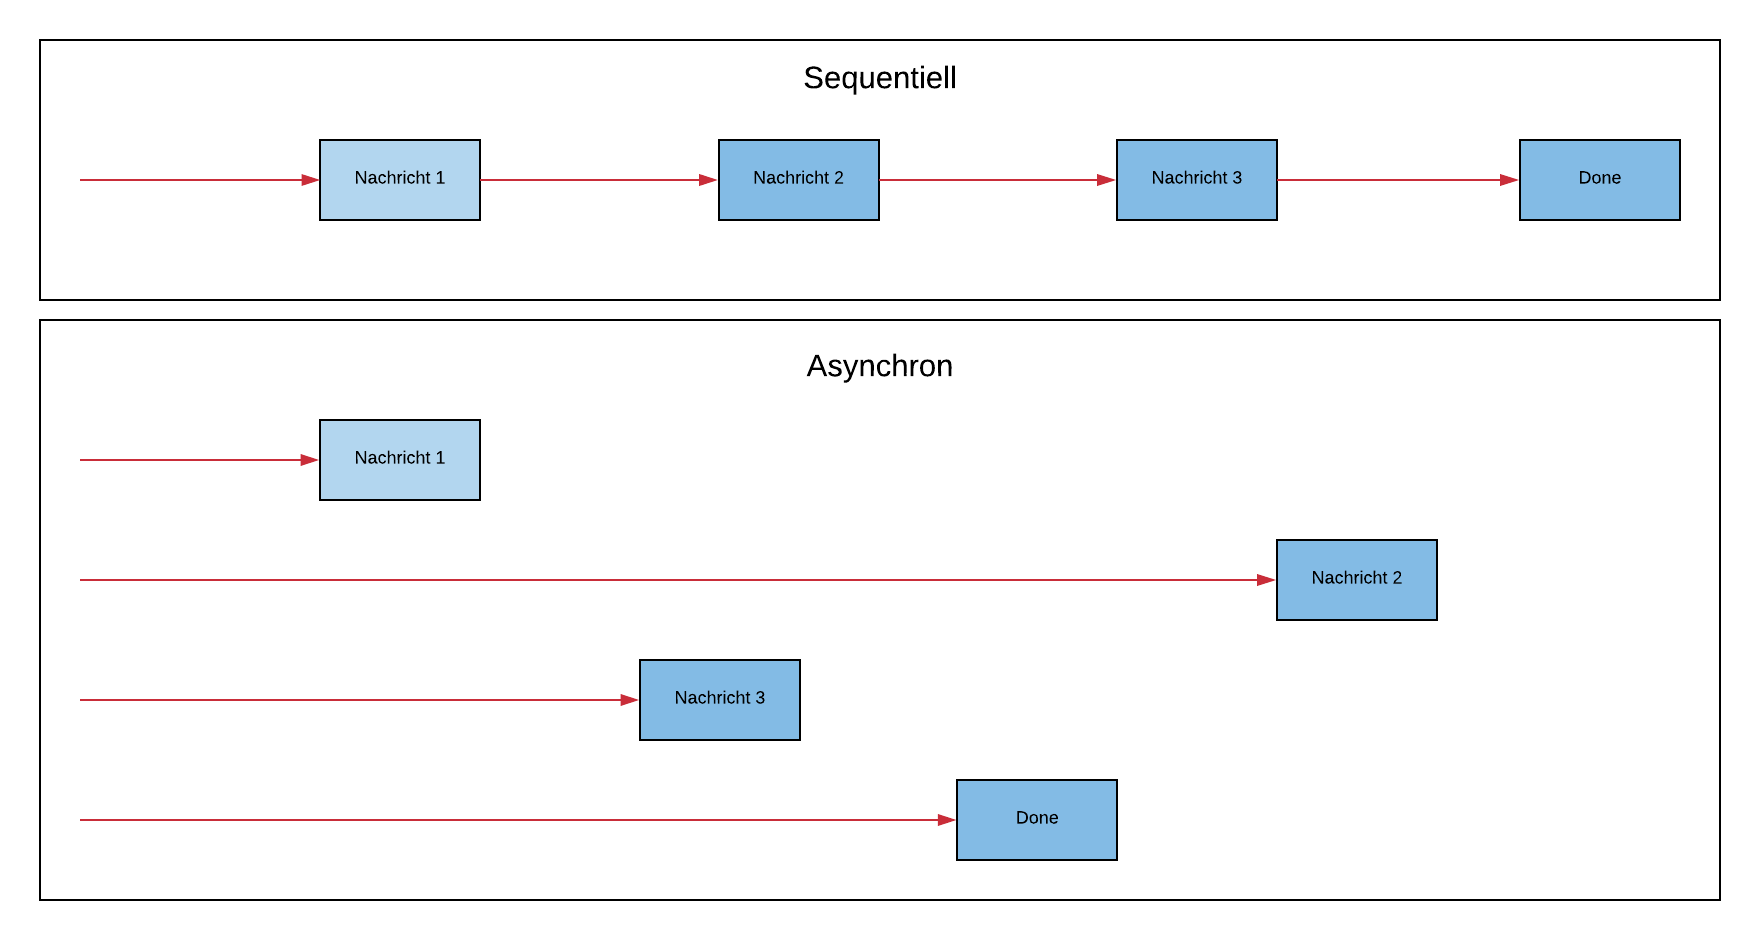
\includegraphics[width=12cm]{synchron-vs-asynchron-diagram}
\caption{Ablauf der ausgeführten Operationen im Browser}
\end{figure}
\end{center}

\noindent
Um zu gewährleisten, dass die Nachrichten trotz Verzögerung aufeinander warten und somit sequentiell ausgeführt werden, würde der Code so aussehen:

\begin{figure}[H]
\begin{lstlisting}
    public printAsyncAndSequential(): void {
        setTimeout(() => {
            this.msg('Hey Im message Nr. 1 !');
            setTimeout(() => {
                this.msg('Hey Im message Nr. 2 !');
                setTimeout(() => {
                    this.msg('Hey Im message Nr. 3!');
                    setTimeout(() => {
                        this.msg('Done!');
                    }, Math.random() * 10);
                }, Math.random() * 10);
            }, Math.random() * 10);
        }, Math.random() * 10);
    }
\end{lstlisting}
\caption{Es bildet sich ein sog. Baum, der sich immer weiter nach rechts ausbreitet.}
\end{figure}

\noindent
Hier werden mehrere Level von Callback-Funktionen ineinander geschachtelt, um die Abhängigkeiten der Aufrufe zu wahren. Sollte jetzt bei einer selbsterstellten Callback-Funktion ein zusätzliches Error-Handling berücksichtigt werden, wird die Nachvollziehbarkeit einer höherrangigen Funktion kaum noch gewährleistet. Der Code oben wird deshalb auch als Callback-Hell bezeichnet.




